\documentclass{article}
\usepackage{v-problem}
\vgeometry
\usepackage{v-electrostatics}

\begin{document}
\vtitle[ELECTROSTATICS]

\def\pn{10}
\def\book{Irodov}
\def\page{106}
\def\gdrive{https://drive.google.com/drive/folders/1ubVlMthM4dO-OrolMaImp6lveHhwJ-HE?usp=share_link}

\def\question{
A thin wire ring of radius $r$ carries a charge $q$. Find the magnitude of the electric field strength on the axis of the ring as a function of distance $l$ from its centre. Investigate the obtained function at $l\gg r$. Find the maximum strength magnitude and the corresponding distance $l$. Draw the approximate plot of the function $E(l)$.
}

\vspace*{\fill}
\begin{tikzpicture}
	\node[qnumber] (n) at (0, 0)[scale=2] {$\pn.$};
	\node[question] (q) [right=2mm of n.east] {\question};
	\tzline[divider]<-0.125, 0> (q.north west)(q.south west);
	\node[format] (f) at  (q.south east){[\book \quad \page]};
\end{tikzpicture}	
\vspace*{\fill}

\begin{center}
\begin{tikzpicture}
\tzcoor*(0, 0)(O){$O$}[b]
\tzcoor*(3, 0)(X)
\tzcoor*(-3, 0)(X')
\foreach \a in {0, 10, ..., 360}{
	\tzcoor(cos{(\a)}, 2.5*sin{(\a)})(P)
	\tznode(P){$+$}[scale=0.8]
	\tzdot(P)(7pt)
	\tzline[->, red]($(P)!0.03!(X)$)($(P)!1.3!(X)$)
	\tzline[->]($(P)!0.03!(X')$)($(P)!1.3!(X')$)
}
\tzline[<->](-5, 0)(5, 0)
\end{tikzpicture}
\end{center}

\pagebreak

\vtitle[\texttt{Solution}]
\begin{center}
\begin{tikzpicture}
[thick]
\tzcoor*(0, 0)(O){$O$}[b]
\tzcoor*(3, 0)(X)
\tzcoor*(-3, 0)(X')
\foreach \a in {0, 10, ..., 360}{
	\tzcoor(cos{(\a)}, 2.5*sin{(\a)})(P)
	\tznode(P){$+$}[scale=0.8]
	\tzdot(P)(7pt)
}
\tzline[<->](-5, 0)(5, 0)
\def\A{6} %angle for element
\def\AA{125} %at angle
\def\r{2.5} %radius
\def\dr{0.15} %delta r
\def\RO{\r+\dr} %radius outer
\def\RI{\r-\dr} %radius inner
\def\R{1.25}
\tzcoor(3, 0)(O') %point at right end
\tzcoor(cos{\AA}, 2.5*sin{\AA})(L)
\tzcoor(1.15*cos{(\AA-\A)}, 2.65*sin{(\AA-\A)})(A)
\tzcoor(1.15*cos{(\AA+\A)}, 2.65*sin{(\AA+\A)})(B)

	\tzlines(O)(A)(O)(B);
	\tzarc(O)(\AA-\A:\AA+\A:{1+\dr} and {\r + \dr})
	\tzarc(O)(\AA-0.5*\A:\AA+2*\A:{1-\dr} and {\r - \dr})
	\tzline[->](L)($(L)!1.25!(O')$){$\d{\vec{E}}$}[r]
	\tzline[|<->|]<0, -0.5>(O)(O'){$l$}[mb]
\end{tikzpicture}
\end{center}

\addtolength{\jot}{3ex}
\begin{align*}
\intertext{Electric field along the y-axis}
\d{E}_y &= \d{E}\times\sin\theta\\
\intertext{Symmetricity will cancel each other}
E_y &= 0\\
\intertext{Electric field along the x-axis}
\d{E}_x &= \d{E}\times\cos\theta\\
		&= \K\cdot \dfrac{\d{q}}{(r^2+l^2)} \cdot \dfrac{l}{\sqrt{r^2+ l^2}}\\
E_x	&=  \K \cdot \dfrac{l}{(r^2+l^2)^{3/2}} \int_0^q \d{q}\\
E_x	&=  \K \cdot \dfrac{ql}{(r^2+l^2)^{3/2}} \\
\intertext{For $l\gg r \Rightarrow r^2/l^2 \approx 0$}
E_x	&= \K \cdot \dfrac{ql}{l^3\left(\dfrac{r^2}{l^2}+1\right)^{3/2}}\\
\Aboxed{E_x &\approx\K \cdot \dfrac{q}{l^2}}
\end{align*}

\pagebreak

\begin{align*}
\intertext{For $E$ to be maximum}
\dfrac{\d{E}}{\d{l}} &= 0\\
\dfrac{\d{E}}{\d{l}} &= \K \cdot \dfrac{\left(r^2+l^2\right)^{3/2}\cdot q-ql\cdot\dfrac{3}{2}\left(r^2+l^2\right)^{1/2}\cdot 2l}{\left(r^2+l^2\right)^3}
\end{align*}
\begin{align*}
\left(r^2+l^2\right)^{3/2}\cdot q-ql\cdot\dfrac{3}{2}\left(r^2+l^2\right)^{1/2}\cdot 2l &= 0\\
\left(r^2+l^2\right)-l\cdot\dfrac{3}{2}\cdot 2l &= 0\\
r^2 - 2l^2 &= 0\\
l &= \dfrac{r}{\sqrt{2}}
\end{align*}

\pagebreak

\begin{align*}
\intertext{Maximum $E$ at $l = \dfrac{r}{\sqrt{2}}$}
E_{\textit{max}} &= \K \cdot \dfrac{ql}{(r^2+l^2)^{3/2}} \\
	&= \K \cdot \dfrac{q\cdot \dfrac{r}{\sqrt{2}}}{\left(r^2+\left(\dfrac{r}{\sqrt{2}}\right)^2\right)^{3/2}}\\
\Aboxed{E_{\textit{max}} &= \dfrac{q}{6\sqrt{3}\pi\varepsilon_0 r^2}}
\end{align*}
\pagebreak

\vspace*{\fill}
\begin{center}
\begin{tikzpicture}
\tzaxes(-5, -3)(5,3){$l$}{$E$}
\def\Fx{4*\x/(1+(\x)^2)^(3/2)}
\tzfn{\Fx}[-5:5]
\tzvXpointat{Fx}{0.707}(A)
\tzproj*[<->,solid,draw=red](A){$l/\sqrt{2}$}{$E_{\textit{max}}$}
\end{tikzpicture}
\end{center}
\vspace*{\fill}
\pagebreak


\vspace*{\fill}
\begin{center}
	\fbox{\qrcode[height=2cm]{\gdrive}}
\end{center}
\vspace*{\fill}

\end{document}
